\chapter{Elastic Scatter of \texorpdfstring{$^8$B}{Boron-8} Solar Neutrinos in \texorpdfstring{\snop}{SNO+}}
\label{ch:es}

During the water phase of {\snop}, after the upgrades made to the SNO detector were commissioned, the detector operated stably for a period of time, producing a physics dataset.
Because of its depth, {\snop} has much lower cosmic muon flux than other water Cherenkov detectors, so even though it is much smaller than, for instance, Super-Kamiokande, it is able to make competitive measurements of nucleon decay~\cite{nucleon_decay} because of lower cosmogenic backgrounds.
These very low backgrounds also enable measurements of solar neutrinos down to low energy thresholds.
The analysis described here does just that by performing a measurement of the $^8$B solar neutrino flux using the elastic scatter (ES) interaction channel.
This represents the first physics results from the {\snop} detector, and also serves as a cross check that {\snop} is correctly simulating its direction resolution.

\section{Introduction}
\label{sec:solar:intro}

{\snop}'s water phase differs from SNO in that light water is used instead of heavy water.
This means that there is no CC or NC interaction, however, there are still electrons present, so the ES process is unchanged.
As described in earlier chapters, the final state electron in the ES interaction has a direction highly correlated with the incident neutrino direction, and this fact can be used to statistically identify ES events in the detector.
This can be achieved by binning events in the observable $\cos{\theta_{sun}}$ which is the cosine of the angle between reconstructed event direction and the Sun at the time of the event.
A maximum likelihood fit similar to the approach described in \Cref{fit_impl}, but using this reduced observable space, can then be performed to extract the observed flux.

\subsection{Solar ES Signal}
\label{sec:solar:inputs}

As with other maximum likelihood fits, PDFs for the solar events must be generated.
The SNOMAN package used to model and analyze data from SNO is replaced by the RAT Monte Carlo and analysis package for {\snop}.
Both operate very similarly: interactions can be simulated in a detailed model of the detector, and PMT hit information can be used to reconstruct events in the same manner as data.
This information is used to build PDFs for statistical analysis of detector data.

Both $\nu_e$ and $\nu_a$ ($\nu_\mu$ and $\nu_\tau$) events are generated with a known flux and flat ($100\%$) survival/transition probability.
This is done for the same reason as in SNO analyses: the neutrino oscillation model is applied as part of the analysis by reweighting events.
The code from the neutrino lifetime analysis presented earlier was leveraged here to produce survival probabilities shown in \Cref{fig:solar:msw} corresponding to the most up-to-date neutrino parameters available from the Particle Data Group~\cite{pdg}.

\begin{figure}
\centering
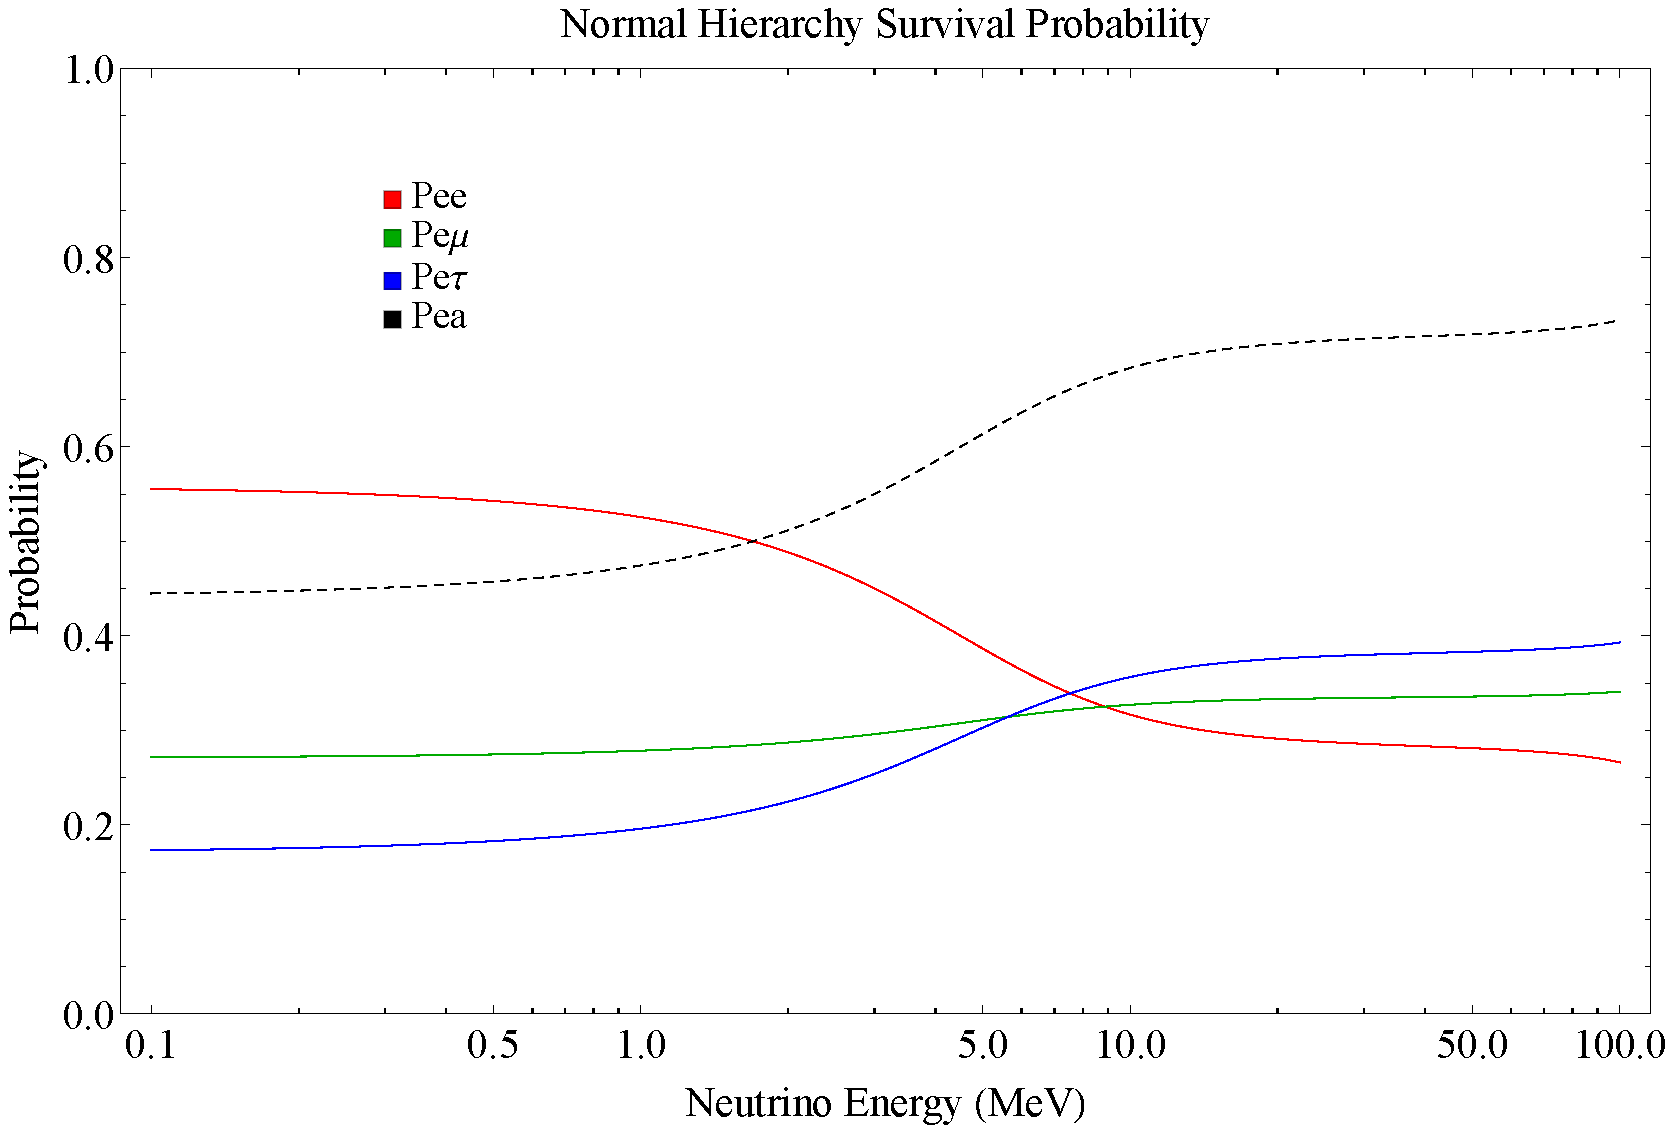
\includegraphics[width=0.8\textwidth]{normal_survival_b8density}
\caption{The MSW survival probability curves used in the {\snop} ES analysis.}
\label{fig:solar:msw}
\end{figure}

Each simulated event is weighted by either $P_{ee}$ for $\nu_e$ or $P_{ea}$ for $\nu_a$ as they are added to a PDF to incorporate known effects of neutrino oscillation.
The relative weights of $\nu_e$ and $\nu_a$ in the PDF are determined by the ES cross section.
RAT MC was generated with the $^8$B flux from BS05(OP)~\cite{bs05op}, but this was rescaled to a more up-to-date measured value~\cite{GlobalSolarFlux}.
Example PDFs can be seen in \Cref{fig:solar:pdfs}.

\begin{figure}
\centering
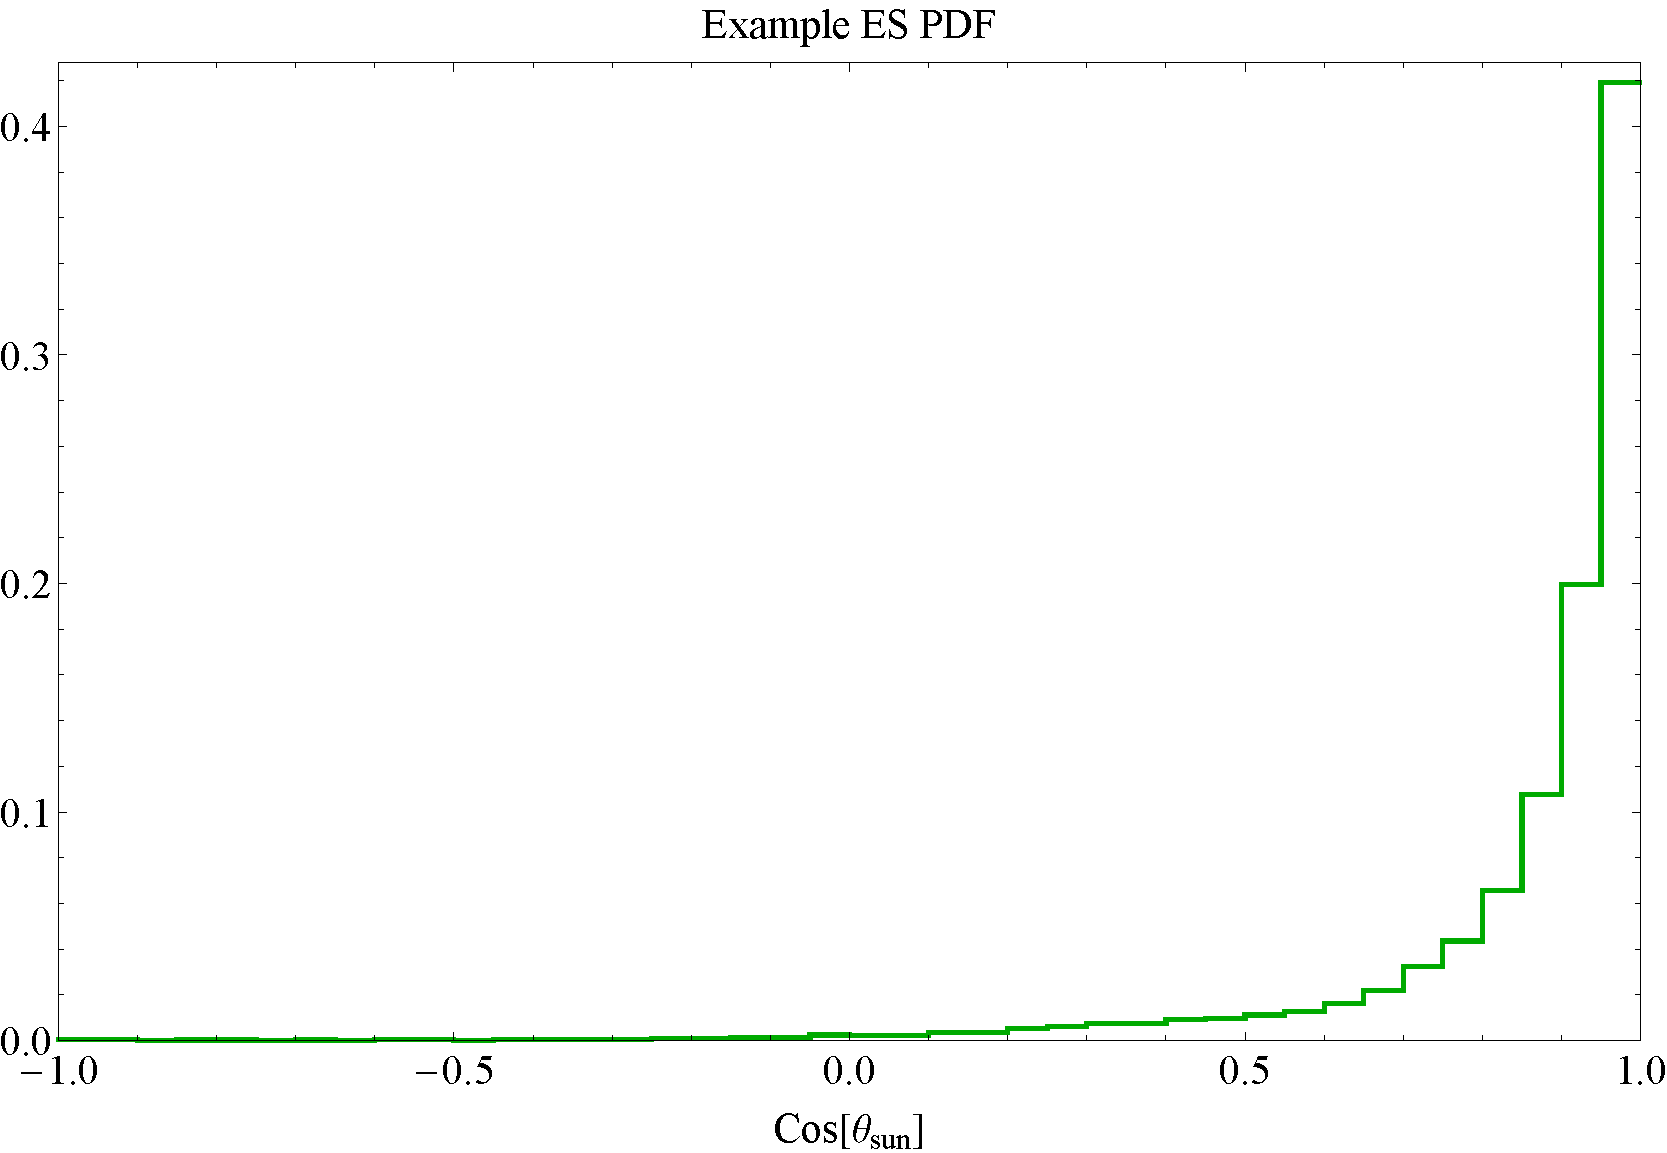
\includegraphics[width=0.8\textwidth]{example_pdf}
\caption{Example PDF for the ES interaction in {\snop}.}
\label{fig:solar:pdfs}
\end{figure}

\subsection{Backgrounds}

Since this analysis is only using the observable $\cos{\theta_{sun}}$, the handling of backgrounds is quite simple.
In short, no other types of event are expected to be correlated with the direction of the Sun, so a flat PDF can be used.
This is demonstrated by generating background PDFs as shown in \Cref{fig:solar:backgrounds} of all backgrounds considered for {\snop}.
Notably, all backgrounds are flat in $\cos{\theta_{sun}}$ as expected.
Using MC derived PDFs offers no benefit here, so an analytically flat PDF is assumed.

\begin{figure}
\centering
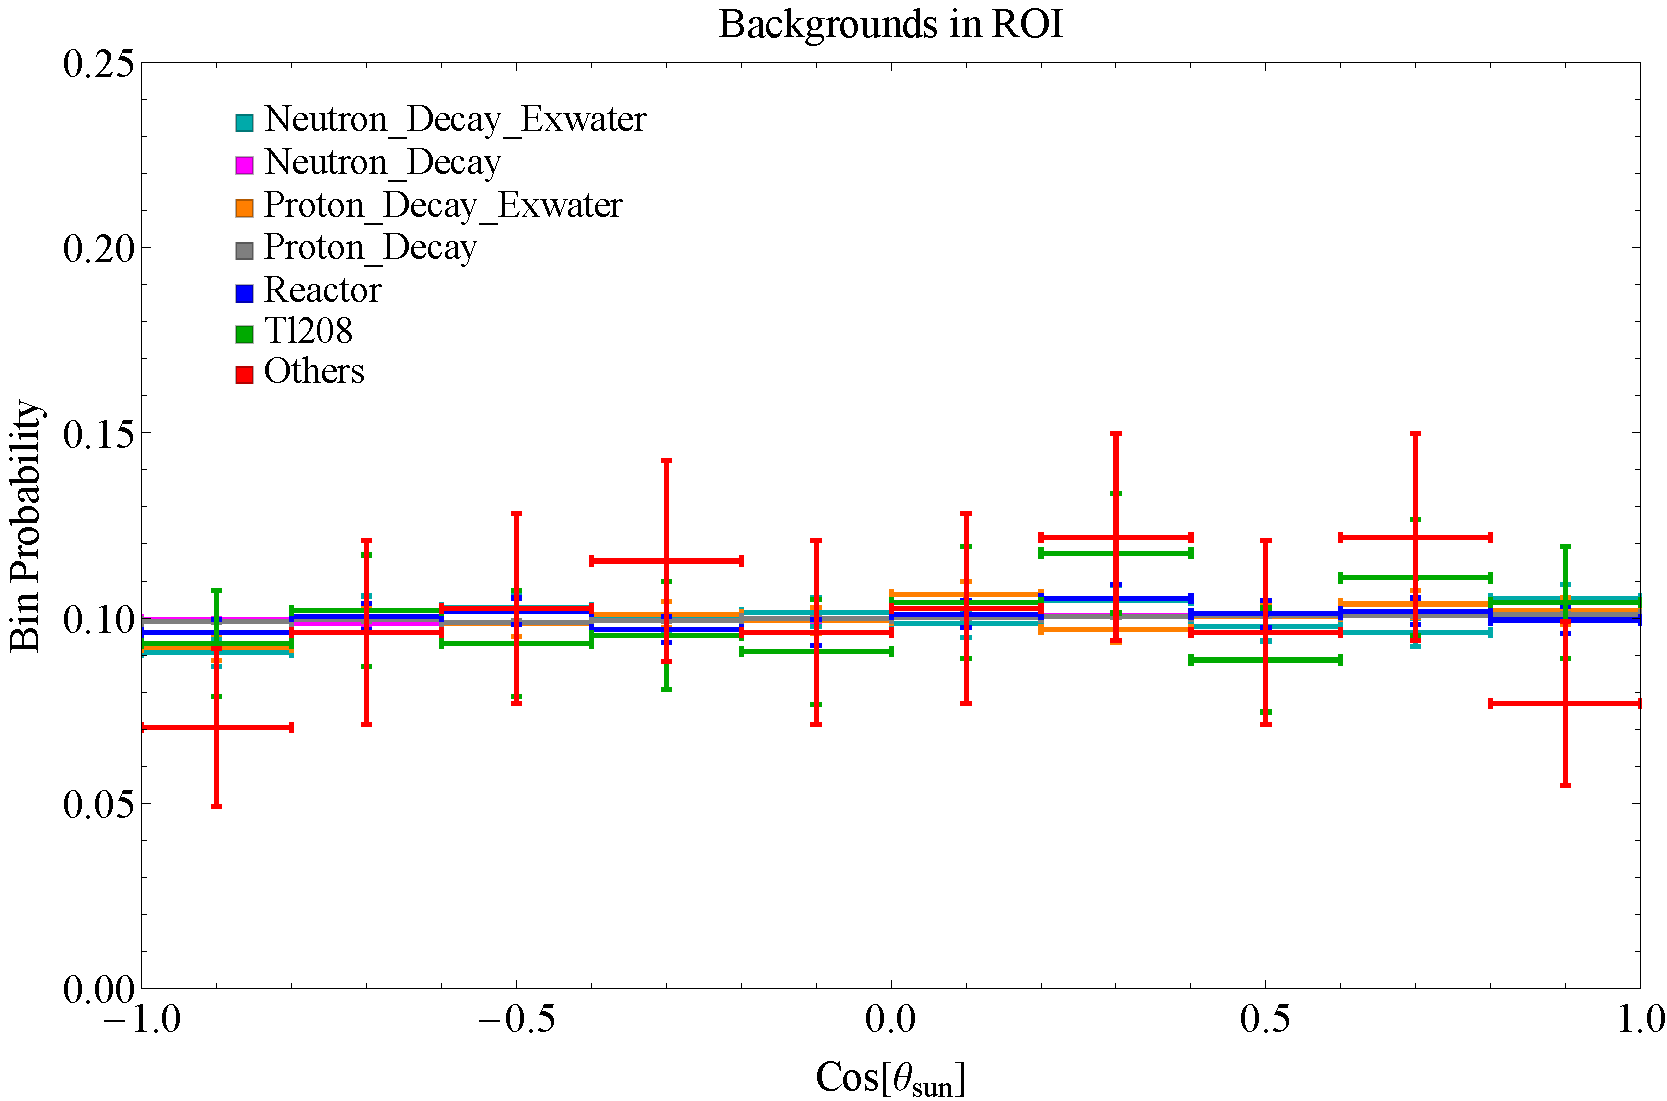
\includegraphics[width=0.8\textwidth]{backgrounds_roi}
\caption{Backgrounds shown binned in the observable $\cos{\theta_{sun}}$ after solar analysis cuts are applied.
Note that backgrounds with fewer than 100 counts were combined and shown as as other.}
\label{fig:solar:backgrounds}
\end{figure}

\clearpage 

\section{Reconstructed Energy Correction}

Careful inspection of energy reconstruction in MC demonstrated that the energy reconstruction algorithm initially applied to real and simulated data contained significant biases at low energies.
It was impractical to correct the algorithm and re-run energy reconstruction on all data (real or simulated), so instead a method to correct the reconstructed values to produce an unbiased estimate of the reconstructed energy was adopted.
By simulating particles of known energies in MC, it was possible to calculate the bias in reconstructed energy as a function of reconstructed energy, and this was used to generate a lookup table to correct for the energy bias.
The lookup table is shown in \Cref{fig:energy_lookup}.

\begin{figure}
\centering
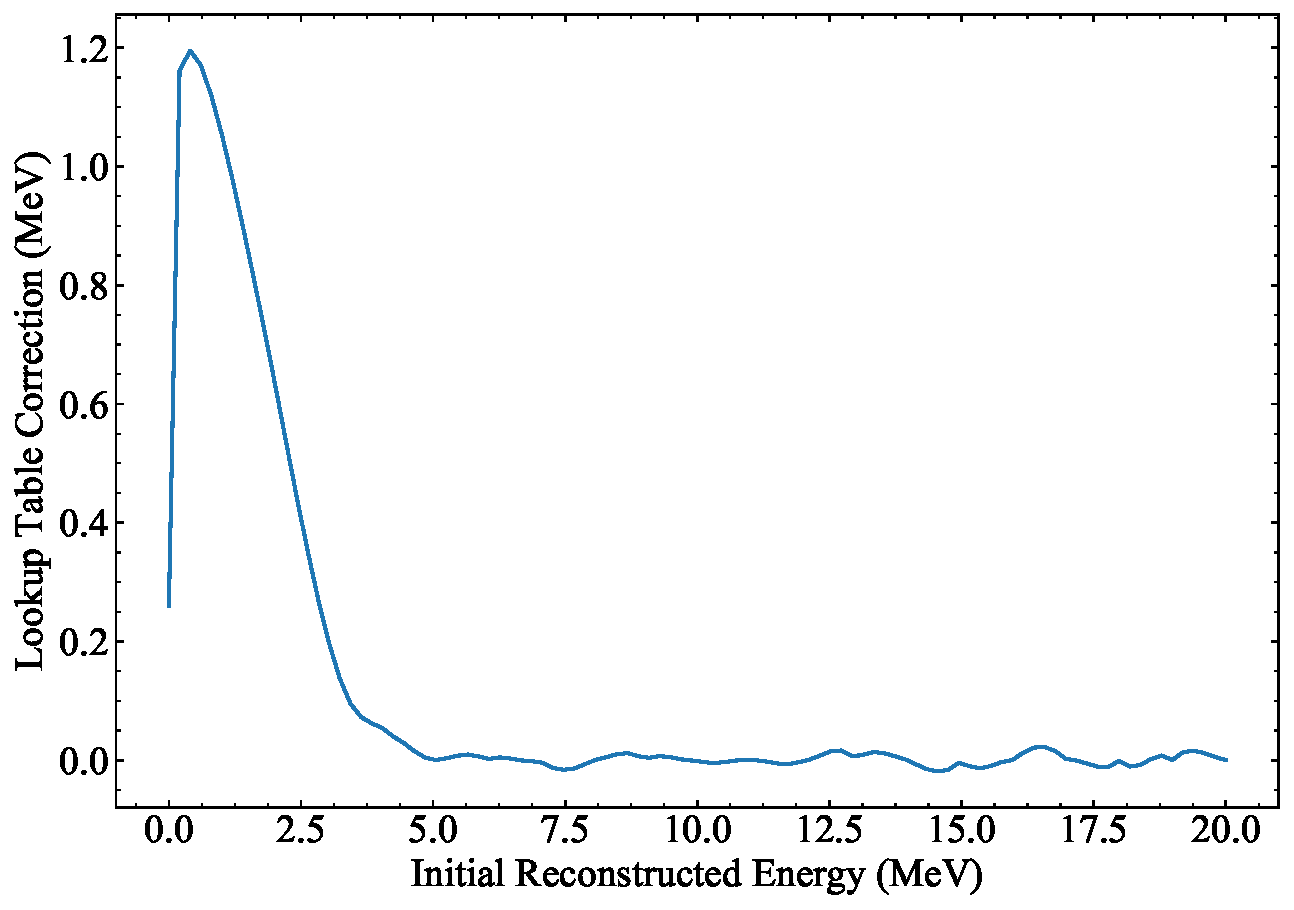
\includegraphics[width=0.8\columnwidth]{energy_correction}
\caption{\label{fig:energy_lookup}The lookup table used in the first step of correcting reconstructed energy in {\snop}. This plot shows the residual of the correction, and applies to both real and simulated data.}
\end{figure}

Further analysis of \N calibration data taken at many locations within the detector demonstrated radius- and z-dependent energy scale bias.
The second correction accounted for this bias separately in real and simulated data by applying a scale factor to the reconstructed energy of the form
\begin{equation}
1 + A + ( (1 + B \rho^2)(1 + Cz + Dz^2 + Ez^3) - 1 )
\end{equation}
where $A$, $B$, $C$, $D$, and $E$ are constants defining the correction.
The values for each constant are summarized in \Cref{tbl:energy_correction}.
After these corrections were applied, the MC was found to well reproduce the \N calibration data throughout the detector.

\begin{table}
\centering
\begin{tabular}{c|l|l}
& Real Data & Simulated Data \\ \hline
A & 2.53e-2 & 3.33e-2 \\ \hline
B & 1.15e-9 & 9.48e-10\\ \hline
C & -5.45e-6 & 3.76e-6\\ \hline
D & 2.14e-9 & 4.46e-10 \\ \hline
E & 6.49e-13 & 1.43e-13
\end{tabular}
\caption{\label{tbl:energy_correction}Coefficients used to further correct the reconstructed energy of {\snop} data according to \Cref{tbl:energy_correction}. This was done separately for real and simulated data after the lookup table in \Cref{fig:energy_lookup} was applied.}
\end{table}

\section{Data Selection}

As this is an early look at {\snop} data, the criteria defining which events are physics and should be analyzed are not as well defined as they are for contemporary analyses of SNO data.
This section discusses these criteria in detail, and aims to produce a set of data free of instrumental backgrounds by defining low level cuts on detector behavior and basic event information, and high level cuts on reconstructed quantities.

For {\snop}, the data within the water phase were separated into various time bins roughly correlated to the background levels during data taking.
The data were split into six datasets, during each of which the background levels were relatively stable, each with its  own  background  estimate  and  set  of  analysis cuts.
For this analysis, where all backgrounds are treated as analytically flat PDFs, changing backgrounds are not a concern.
Of relevance are the variation of analysis cuts between the six datasets, which must be accounted for in the analysis.
These data selection criteria described in the following sections were also applied in the process of building PDFs to MC simulation for each time bin to correctly account for the varying acceptance these different cuts imply.

\subsection{Low-Level Cuts}

The {\snop} trigger system records a 32~bit integer where each bit is a boolean mask of the state of the trigger system for each event.
This trigger word identifies, at a very low level, what caused the detector to take data.
Low-level event selection requires that the trigger word include a physics trigger based on the number of coincidentally hit PMTs, and excludes any externally forced triggers that may be in the data.
Externally forced triggers include a periodic trigger that is used to monitor the noise rates in the detector, triggers related to deployed sources, and diagnostic triggers issued by the detector electronics for self-testing.
None of these external triggers represent valid data for analysis and must be excluded.

Various data cleaning classifiers are run over the raw data as part of reconstruction, with the goal of identifying instrumental backgrounds, or other non-physics events, that survive other cuts.
These classifiers produce another 32~bit word which can be checked for event quality.
A check of the data cleaning word requires that all standard data cleaning classifiers did not mark the event as dirty.
These classifiers seek to exclude cosmic muons, cosmic muon follower events, flashes of light from PMTs that have similar topology to Cherenkov events, and other features of the data that can be identified.
These classifiers are also run on simulated data, and the signal sacrifice is estimated and accounted for. 

\subsection{High-Level Cuts}

Once an event satisfies low-level event selection criteria, the results of event reconstruction can be considered.
A valid reconstruction result is required, meaning the reconstruction algorithms successfully converged to some value.
High level cuts are applied on the in-time ratio (ITR), representing the ratio of number of hit PMTs within a prompt time window to all hit PMTs, and isotropy ($\beta_{14}$), representing the isotropy of the pattern of hit PMTs.
These two metrics were both used in SNO to remove instrumental backgrounds, as described in \Cref{sec:sno_observables}, since Cherenkov events are expected to have a very sharp time signature and produce events consistent with Cherenkov light topology.

The region of interest (ROI) for the analysis is then selected with cuts on energy and radius.
Note that initially this analysis only planned to extend down to 5.5~MeV, however, evaluation of the actual data indicated that backgrounds were low enough to consider events down to 5.0~MeV.
Other analyses of this data identified a region of high radioactivity near the top of the detector, and for this a z dependent radial cut was adopted.
These high level cuts are summarized per time bin in \Cref{tbl:solar:roi}.

\begin{table}
\begin{center}
\begin{tabular}{l|c|c|c}
\textbf{Time Bin} & I & II & III  \\ \hline
\textbf{Run Range} & 100000-100399 & 100400-102048 & 102049-103402 \\ \hline
\textbf{Criteria} & ITR $ \geq 0.55$ & ITR $ \geq 0.55$ & ITR $ \geq 0.55$ \\
& $-0.12 \leq \beta_{14} \leq 0.95$ & $-0.12 \leq \beta_{14} \leq 0.95$ & $-0.12 \leq \beta_{14} \leq 0.95$ \\
& $5.0 \leq E \leq 15.0$ & $5.0 \leq E \leq 15.0$ & $5.0 \leq E \leq 15.0$ \\
& $R \leq 5.3$ & $R \leq 5.3$ (for Z$<$0) & $R \leq 5.3$ \\
& & $R \leq 4.2$ (for Z$>$0) & \\
\end{tabular}
\\[2\baselineskip]
\begin{tabular}{l|c|c|c}
\textbf{Time Bin} & IV & V & VI \\ \hline
\textbf{Run Range} & 103411-105171 & 105493-105661 & 106716- \\
& & 106070-106499 & \\ \hline
\textbf{Criteria} & ITR $ \geq 0.55$ & ITR $ \geq 0.55$ & ITR $ \geq 0.55$ \\
& $-0.12 \leq \beta_{14} \leq 0.95$ & $-0.12 \leq \beta_{14} \leq 0.95$ & $-0.12 \leq \beta_{14} \leq 0.95$ \\
& $5.0 \leq E \leq 15.0$ & $5.0 \leq E \leq 15.0$ & $5.0 \leq E \leq 15.0$ \\
& $R \leq 5.3$ & $R \leq 5.3$ & $R \leq 5.3$ \\
\end{tabular}
\caption{The high level cuts used in the {\snop} ES analysis. Selected events will pass these cuts.}
\label{tbl:solar:roi}
\end{center}
\end{table}


\section{Systematic Uncertainties}

With the procedure described above for generating signal and background PDFs, the extended maximum likelihood fit is straightforward.
The remaining concern are systematic uncertainties that might be present between the data and simulated events.
For this analysis, systematics are propagated primarily with a shift-and-refit method.

Independent analyses of \N calibration data produce central values and uncertainties for each systematic uncertainty.
The fit is run with systematics fixed at their central values to obtain the central results of the fit.
Each systematic is then independently shifted by its one-sigma uncertainty, the fit re-run, and the variation of the shifted results with respect to the central fit results is taken as the systematic uncertainty on the results.
As a final step, the variations from all systematics are combined in quadrature to arrive at the total systematic uncertainty.
This assumes that systematic uncertainties are uncorrelated and their effects normally distributed.

The following sections describe in detail each systematic considered.

\subsection{Energy Scale and Resolution}

The energy scale and resolution were determined by comparing data from a deployment of the \N calibration source to MC. 
This yielded a $2.9\%$ uncertainty on the energy scale, and required an additional $10.2\%$ smearing at $5$MeV to be applied to MC to match the data.
To find the smearing at other energies $E$ in MeV, the following equation was assumed
\begin{equation}
\label{eqn:solar:esmear}
E_{smear} = 0.102\sqrt{5 E}.
\end{equation}

To propagate the energy scale systematic, the MC reconstructed energy was scaled up and down by $2.9\%$ and the analysis performed again with each condition.
The resulting variation in the fitted measured flux was taken as the systematic uncertainty on the flux.
The energy resolution systematic was propagated by smearing the reconstructed MC energies by \Cref{eqn:solar:esmear} and then rerunning the fit.
Again, the resulting variation in the measured flux is taken as the systematic uncertainty.

\subsection{Position Scale and Resolution}

As the solar MC is simulated as a uniform distribution inside the AV, and the position resolution of {\snop} is small (approximately 10~cm), smearing the reconstructed position by this resolution has a negligible effect on the expected number of events.
However, this uncertainty is propagated similar to the energy resolution systematic: by smearing the MC reconstructed positions by the position resolution and rerunning the analysis.
The more important position systematic is the position scale, as this changes the fiducial volume which is directly proportional to the measured flux.
The vertex scale systematic is determined for each axis by comparing \N data to MC, and found uncertainties of $(^{+0.03}_{-0.19}\%,^{+0.03}_{-0.38}\%,^{+0.03}_{-0.37}\%)$.
To propagate these systematics the axes were simultaneously scaled up and down by these values, and the fit was rerun.

\subsection{Angular Resolution}

The uncertainty in angular resolution was accounted for by remapping the angle between true direction and reconstructed direction, $\cos{\phi}$, using the equation
\begin{equation}
\cos{\phi'} = 1 + \frac{\cos{\phi}-1}{1\pm\Delta}
\label{solar:eq:dirres}
\end{equation}
where $\Delta$ is a parameter representing the systematic uncertainty on the angular resolution.
After adjusting the reconstructed direction of each MC event to be further or nearer the MC truth direction, the $\cos \theta_{sun}$ PDF is recomputed using these new directions.
The fit is then rerun with the new $\cos \theta_{sun}$ PDF to compute the impact of this systematic.

As the angular systematic was determined to be the dominant systematic, and the solar data well constrains the angular resolution, this uncertainty is floated with a constraint determined by independent analysis of \N calibration data.
The constraint on $\Delta$ was determined to be $0^{+0.08}_{-0.19}$.
This requires re-smearing each event's direction and rebuilding the angular PDF at each step of the fit which is computationally challenging but tractable for this analysis with so few floated variables.

\section{Open Data Analysis}
\label{sec:solar:opendata}

To understand detector data, constrain backgrounds, and aid in the development of analyses, {\snop} provided about 16~days of detector livetime with no blinding applied.
The remaining data was withheld until analyses were developed so that unbiased results could be extracted.

\begin{table}
\centering
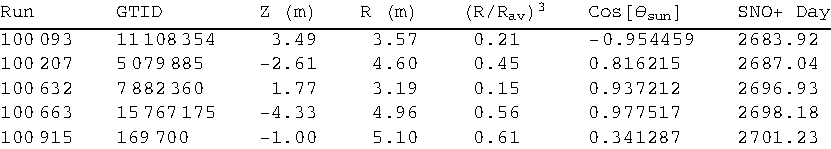
\includegraphics[width=\textwidth]{events}
\caption{The events selected by solar analysis cuts in the open dataset.}
\label{tbl:solar:openev}
\end{table}

The following preliminary diagnostic plots are created with a higher energy threshold of 5.5~MeV.
After applying the data selection criteria to this open data, there are 5 candidate ES events selected.
These candidates are shown with various observables in \Cref{tbl:solar:openev}.
The {\snop} date for the runs included along with the 5 selected events is shown in \Cref{fig:solar:opendata} to gain confidence that these events are not suspiciously distributed in time.
In a similar vein, the time of day of each event along with the relative livetime (represented by number of runs at that time) is shown in \Cref{fig:solar:tod}.

\begin{figure}
\centering
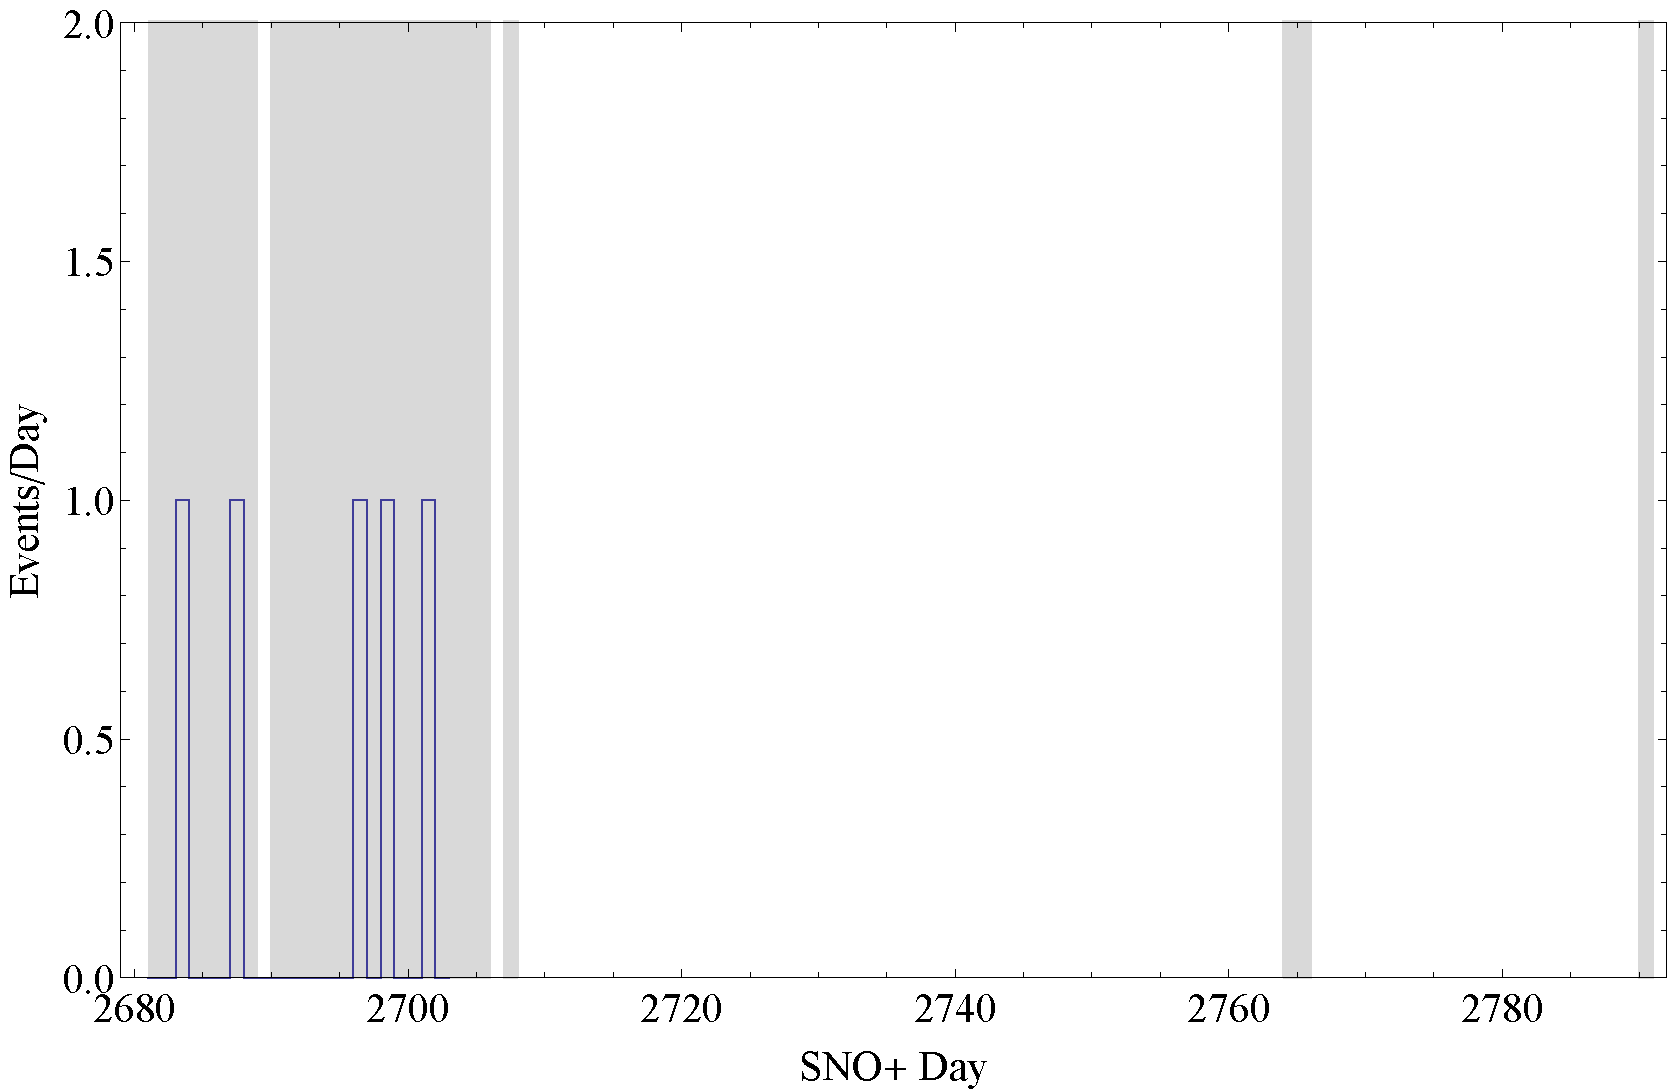
\includegraphics[width=0.8\textwidth]{per_day}
\caption{The {\snop} days that are included in the open data analysis are shown shaded gray.
The date of each selected event in the open data analysis is also shown.}
\label{fig:solar:opendata}
\end{figure}


\begin{figure}
\centering
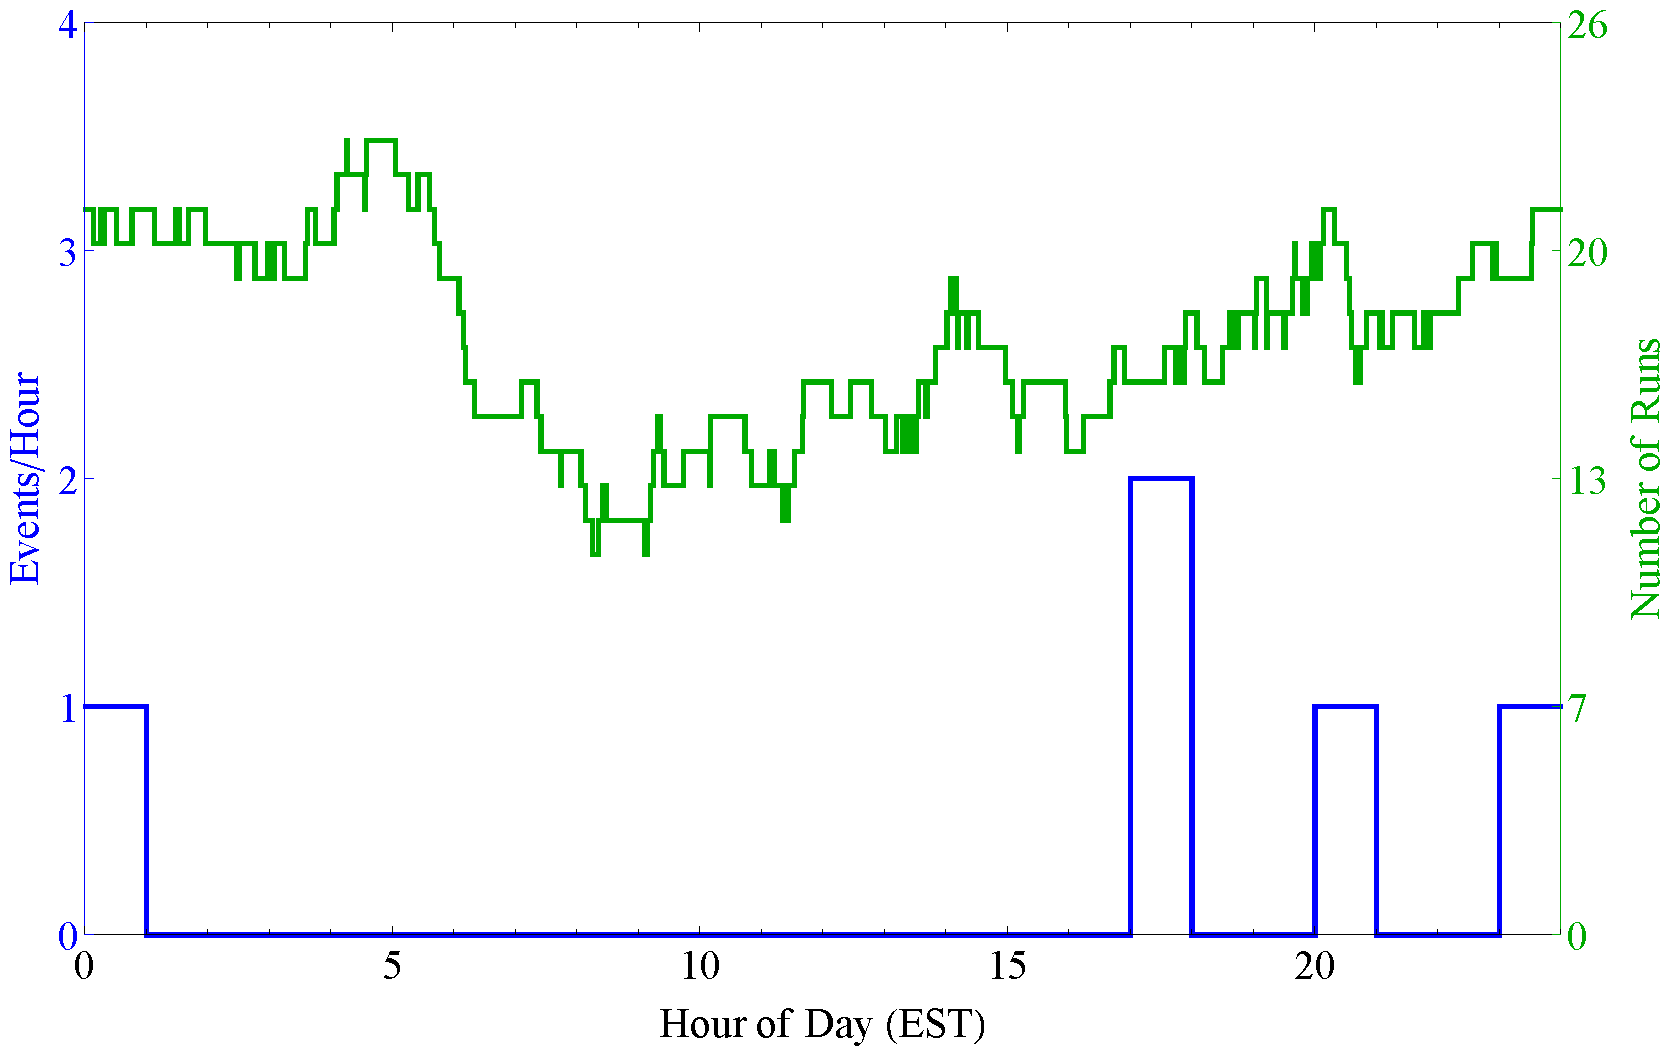
\includegraphics[width=0.8\textwidth]{hour_of_day}
\caption{The time of day (Sudbury timezone, no DST correction) of each selected event in the open data analysis.
Also shown are the number of runs at any particular time of day.}
\label{fig:solar:tod}
\end{figure}


Due to there being so few events in this dataset, a very coarse binning of $0.2$ in $\cos{\theta_{sun}}$ intervals is used.
For the open dataset with a 5.5-MeV threshold, a flux scale of $0.54 \pm 0.37$~(stat.)~$^{+0.09}_{-0.05}$~(syst.) is found.
Flux scale is interpreted as the fraction of the expected $^8$B flux that was observed.
The best fit is shown plotted with the binned data in \Cref{fig:solar:open55}.
While this result disagrees with the expected $^8$B flux at over one sigma, it is expected that this is a statistical fluctuation due to very few statistics.

\begin{figure}
\centering
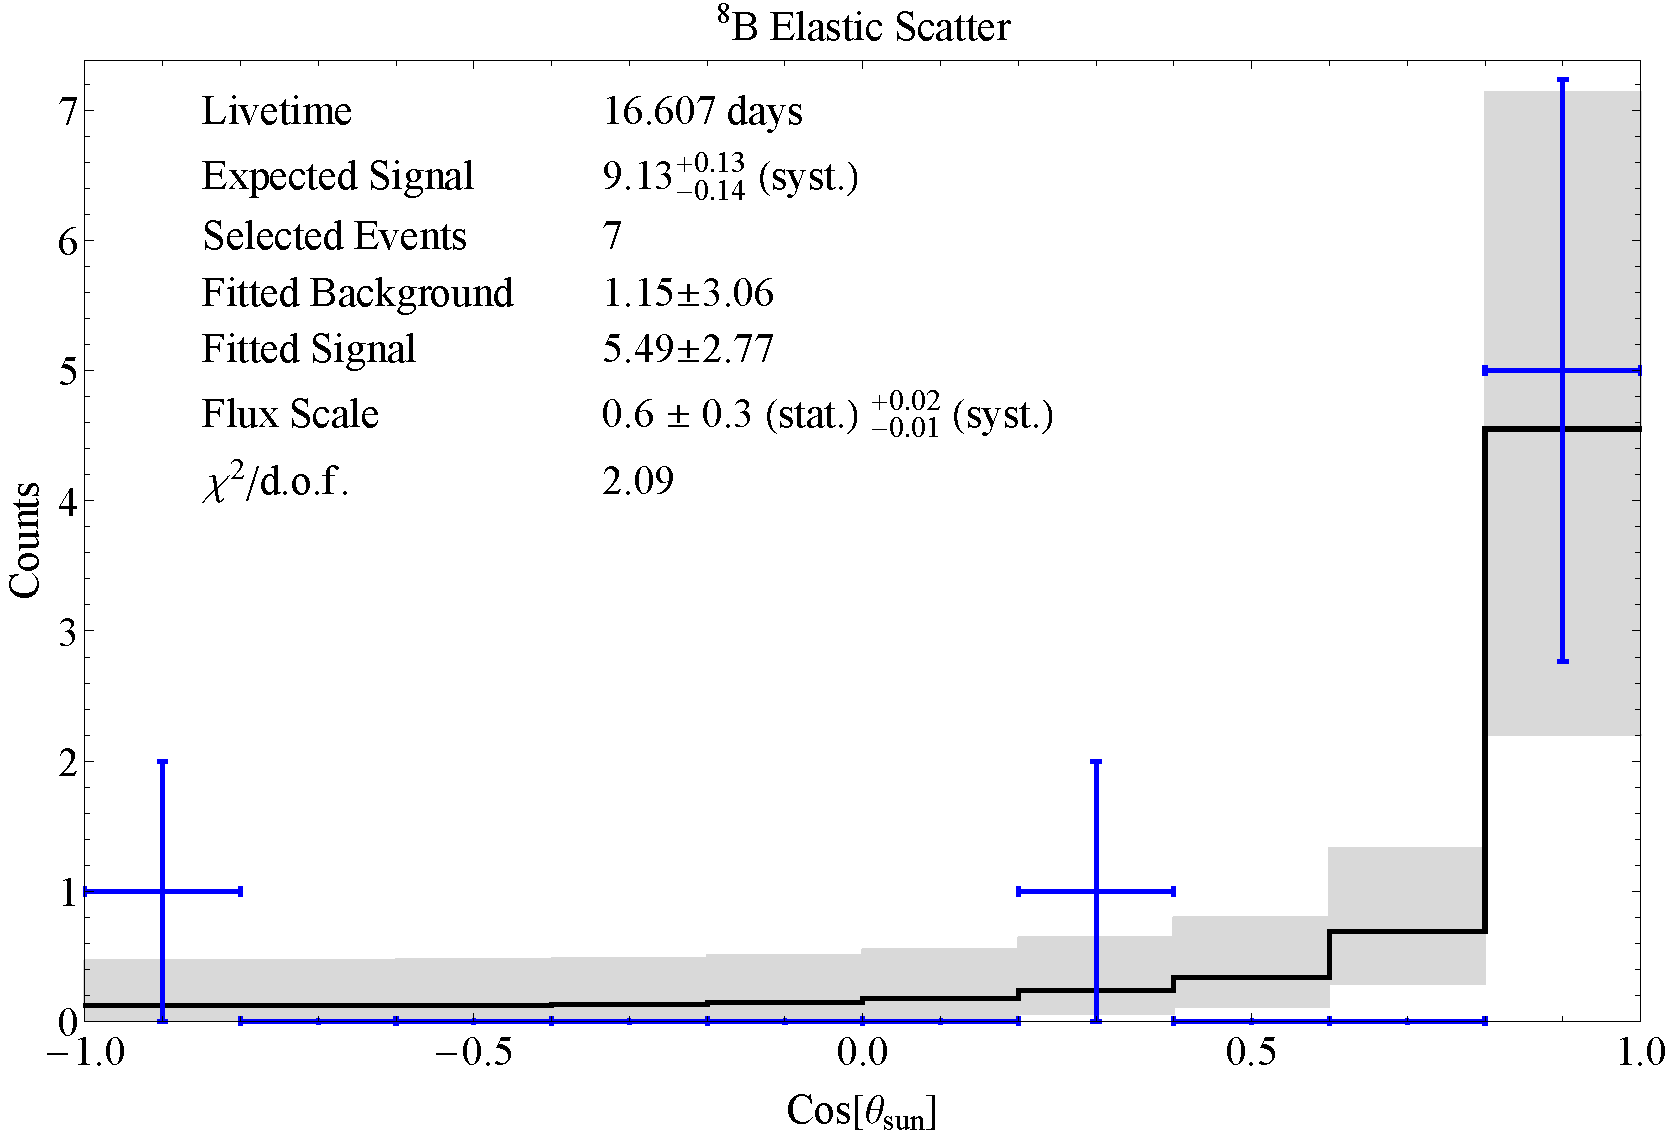
\includegraphics[width=0.8\textwidth]{b8_es_fit_5_5}
\caption{
Summary plot of the $^8$B ES fit on the open dataset using the energy range 5.5-15.0~MeV.
The shaded regions show the fit uncertainty, with the selected events shown in blue.
The fitted flux scale is shown relative to the current global predictions in~\cite{GlobalSolarFlux}.
}
\label{fig:solar:open55}
\end{figure}

\section{Final Results}
\label{sec:solar:updated}

Following a review of the open data analysis as described in the previous section, the {\snop} Analysis Committee approved the analysis procedure to move ahead with the entire {\snop} water phase dataset.
The additional livetime (approximately 115~days) and additional events this implies allows for finer data binning of 0.05 in $\cos{\theta_{sun}}$ intervals.
Further, there are sufficient statistics for this fit to be performed in independent energy bins within the 5.0-15.0~MeV ROI.
This is advantageous because background rates increase as energy decreases, so energy bins at the high end of this range would be less susceptible to statistical fluctuations in the backgrounds.
By multiplying together the marginalized likelihoods as a function of $^8$B flux for each independent fit, a combined likelihood for the total dataset can be obtained.
This combined likelihood results in a better determination of the overall solar neutrino flux than would a fit to the full energy range.
Five bins 1-MeV wide are considered in the range 5.0-10.0~MeV, along with a single bin from 10.0-15.0~MeV.

\begin{figure}
\centering
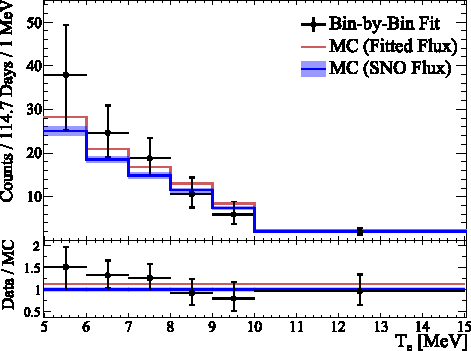
\includegraphics[width=0.75\textwidth]{snoplus_solar_binned}
\caption{The total number of ES events from each energy bin in the {\snop} $^8$B ES analysis is shown in the top panel. 
The bottom panel shows the same information as a ratio to the expected number of ES events from SNO. 
Also shown are the expected number of events from MC when assuming an $^8$B flux as measured by SNO (blue, with uncertainty from the SNO measurement shown as a shaded region), and assuming the best fit of this analysis (red, with uncertainty shown on data).}
\label{fig:solar:binned}
\end{figure}

\begin{figure}
\centering
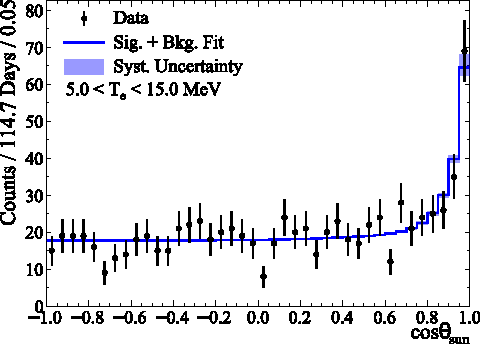
\includegraphics[width=0.8\textwidth]{snoplus_solar_summary}
\caption{The best fit for the {\snop} $^8$B ES analysis, shown with data from the full 5.0-15.0~MeV energy range.}
\label{fig:solar:summary}
\end{figure}

\begin{table}
\begin{center}
\begin{tabular}{c|c|c|c}
Systematic & Uncertainty & Application & Origin \\ \hline
$E_{scale}$     & $\pm 2.0\%$ & shift-refit $^{+0.0217}_{-0.0204}$ & \N \rule{0pt}{2.6ex}\rule[-1.2ex]{0pt}{0pt}  \\
$E_{res}$       & $\sqrt{(1+0.0018)^2-1.0}\sqrt{E}$ & shift-refit $\pm 0.0005$ & \N  \rule{0pt}{2.6ex}\rule[-1.2ex]{0pt}{0pt}  \\
${XYZ}_{scale}$ & $(^{+0.91}_{-1.01},^{+0.92}_{-1.02},^{+0.91}_{-0.99}) \%$ & shift-refit $^{+0.0261}_{-0.0284}$ & \N  \rule{0pt}{2.6ex}\rule[-1.2ex]{0pt}{0pt}  \\
${XYZ}_{shift}$ & $(^{+16.4}_{-18.2},^{+22.3}_{-19.2},^{+38.4]}_{-16.7})$~mm & shift-refit $^{+0.0002}_{-0.0001}$ & \N  \rule{0pt}{2.6ex}\rule[-1.2ex]{0pt}{0pt}  \\
${XYZ}_{res}$ & $(104.0,98.2,106.2)$~mm & shift-refit $\pm 0.0002$ & \N \rule{0pt}{2.6ex}\rule[-1.2ex]{0pt}{0pt}  \\
Dir$_{res}$     &  $\Delta = ^{+0.08}_{-0.13}$ & floated (best fit $\Delta = -0.02^{+0.09}_{-0.13}$) & \N \rule{0pt}{2.6ex}\rule[-1.2ex]{0pt}{0pt}  \\ \hline
\end{tabular}
\caption{ Systematic uncertainties considered on the {\snop} ES analysis are shown here.
The impact shown for shift-and-refit parameters is a fractional change of the $^8$B flux from the central value of the fit for the energy range $5.0-15.0$~MeV.
For the livetime considered in this analysis approximately 100 solar ES events are expected.}
\label{tbl:solar:systs}
\end{center}
\end{table}

Using the full dataset, each energy bin is fit separately.
\Cref{chap:solar_bins} contains the results of each independent fit showing the data in each bin.
The total number of ES events extracted by each of the independent fits is shown in \Cref{fig:solar:binned} relative to previous SNO results~\cite{3phase}, and the best fit $^8$B flux for this analysis: 
\begin{equation}
\Phi_{\mathrm{^8B}} = 5.95^{+0.75}_{-0.71}\mathrm{(stat.)}^{+0.28}_{-0.20}\mathrm{(syst.)} \times 10^6\,\,\mathrm{cm}^{-2}\mathrm{s}^{-1}.
\end{equation}
This $^8$B flux corresponds to an observed flux of ES interactions,
\begin{equation}
\Phi_{\mathrm{ES}} = 2.53^{+0.31}_{-0.28}\mathrm{(stat.)}^{+0.13}_{-0.10}\mathrm{(syst.)} \times 10^6\,\,\mathrm{cm}^{-2}\mathrm{s}^{-1},
\end{equation}
which is in agreement with the Super-Kamiokande result~\cite{superkiv} $\Phi_{\mathrm{ES}} = (2.345\pm0.039)\times 10^6$~cm$^{-2}$s$^{-1}$.
The combined result overlaying the data from the full energy range is shown in \Cref{fig:solar:summary}.
\Cref{tbl:solar:systs} shows in detail the impact of each systematic uncertainty. 
Notably this fit is consistent with the current global best fit for the $^8$B neutrino flux~\cite{GlobalSolarFlux}, $5.16^{+0.13}_{-0.09}$(stat)$^{+0.30}_{-0.26}$(syst)$\times 10^6$~cm$^{-2}$s$^{-1}$.

\begin{figure}
\centering
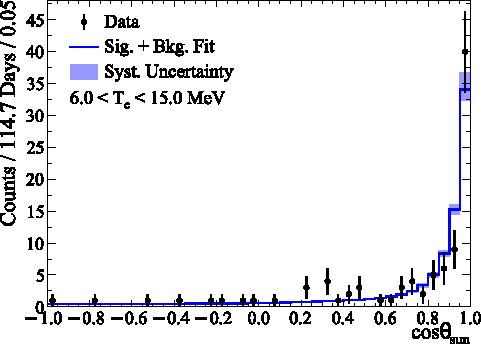
\includegraphics[width=0.8\textwidth]{snoplus_solar_lowbg}
\caption{The fit results from the {\snop} $^8$B ES analysis excluding the lowest energy bin from 5.0-6.0~MeV. Notably, this demonstrates {\snop} has very low backgrounds above 6.0~MeV.}
\label{fig:solar:lowbg}
\end{figure}

The majority of the background events are contained within the 5.0-6.0~MeV energy bin.
With this bin included, the solar neutrino event rate is $1.30\pm0.18$~events/kt-day while the background rate is $10.23\pm0.38$~events/kt-day.
If this bin is excluded, \Cref{fig:solar:lowbg} shows very low backgrounds {\snop} achieved above 6.0~MeV.
For the 6.0-15.0~MeV range the solar neutrino event rate is $1.03\pm0.13$~events/kt-day while the background rate is $0.25\pm0.08$~events/kt-day.
This demonstrates that {\snop} has achieved very low backgrounds above 6.0~MeV, which is an excellent conclusion to arrive at as {\snop} moves into scintillator phase.
